\chapter{Data Aggregation With Internal Verification} % (fold)
\label{cha:Data Aggregation With Internal Verification}
	The most significant design aspect of the sensor network is the \textbf{lifetime of the network}.
	The sensor network tend to have limited life span as they are powered by the battery.
	The lifetime of the sensor network is inversely proportional to the sensor nodes' power consumption.
	One of the most dominating factor for the power consumption is transmitting and receiving the data between sensor nodes, making network bandwidth an expensive resource.
	The bandwidth is more expensive resource than the local data computation, as data computation consumes less power than transmitting or receiving the data.
	The obvious solution to increase the lifespan of the sensor network is to decrease the bandwidth usage in the network.  	
	Data aggregation techniques can reduce the bandwidth usage in the network. 
	It can greatly increase the lifespan of the network.
	Hence, data-aggregation techniques are one of the key tool in our tool box while designing protocol for the sensor networks.

	The second most significant factor in the design of the data aggregation protocol is \textbf{security}. 
	In the perfect world, one desires the following security properties from the secure networking protocol.\\*
	\textbf{Confidentiality} - ensures that information is accessed only by authorized parties.
	% That is, only those who should have access to something will actually get that access. By access, we mean not only reading but also viewing, printing, or simply knowing that a particular asset exists. 
	It is also known as secrecy or privacy.
	Ensuring confidentiality can be difficult.
	For example, who determines which parties are authorized to access the information?
	By ``accessing'' information, do we mean that an authorized party can access a single bit? the whole collection? pieces of information out of context?
	Can someone who is authorized disclose that information to other parties?\cite{pfleeger2002security}
	\\*
	\textbf{Integrity} - assures that the only authorized entities can modify the information; where modification means writing, creating, deleting and changing the information. 
	If one say one have preserved an integrity of the information one may mean different things depending on the context.
	It can mean the following, one has preserved the information is precise, unmodified, modified only in acceptable ways by authorized parties or process.
	Error detection and correction are two important aspects of information integrity \cite{pfleeger2002security}.
	One important application of an integrity is when a user downloads any information from the web, the user wants to be assured that the information has not been altered in any way by the networking errors, by active attackers on the Internet or any other third party application.\\*
	\textbf{Availability} - means that information is accessible to authorized parties at appropriate times.
	In other words, if some person or system has legitimate access to a particular set of objects, that access should not be prevented.
	Availability applies to the information and services.
	For example, information or service is available can mean the following. 
	It is present in the usable form.
	It has the enough capacity to meet the service need.
	It is making enough progress, and, if it is in wait mode, it has a bounded waiting time. There is timely response to our requests.
	Resources are allocated fairly so that some requests are not favored over the others. The service can be used easily and in its intended way.
	For this reason, availability is sometimes known by its opposite, denial of service \cite{pfleeger2002security}.
	\\*
	\textbf{Authentication} - assures the origin of the information.
	There are two types of authentication that rises in cryptography: entity authentication and data-origin authentication \cite{trappe2006introduction}.
	The entity authentication is also known as identification which is concerned with proving the identity of the parties involved in a communication.
	Data-origin authentication focuses on tying the information about the origin of the data, such as the creator and time of creation, with the data.\\*
	\textbf{Non repudiation} - requires neither the sender nor the receiver can deny the transmission.
	This is very important in electronic commerce applications. where it is important that a consumer cannot deny the authorization of a purchase.
	\\*
	\textbf{Access Control} - restricts an access to the information.
	Login credentials and Locks are two analogues mechanism of access control.

	As you can see, expectations from secure networking protocol are far-reaching.
	It is very ambitious for any system to have all the above mentioned security properties at the same time.
	In reality all the security properties are not always required.
	For an instance, when a client downloads a file from the File server using Internet.
	A client can verify the integrity of the File using the checksum.
	But it is okay if somebody on the network sniffed the downloading activity as far as it did not change the content of the File.
	In this application, a client requires the integrity of the File but the privacy of the client, the File server and the Internet service provider are not required.
	To give an analogy with a physical world application, when a person writes a letter in its own handwriting, he puts his own signature on the letter. 
	When that letter reaches to the other end the receiving party can verify the integrity of the message from the handwriting and the signature of the person.
	The postal service knows the sender and the receiver of the letter.
	It can even read the letter if its not in the closed envelop.
	Again, here integrity is important not the confidentiality.

	It is critical to find out which security properties are desired for the particular application.
	In practice, protocol designer finds out the most important security properties for the applications before designing the protocol.

	For example, Wagner's work \cite{wagner2004resilient} describes the attacks on standard schemes for data aggregation and introduces the problem of securing aggregation in the presence of malicious or spoofed data.
	He proposes a mathematical theory of security for aggregation.
	The theory quantifies, in a principled way, the robustness of an aggregation operator against malicious data.
	It draws novel connections to statistical estimation theory and to the field of robust statistics.
	He identifies techniques for aggregation that provide robustness against attack. 
	It provides helpful guidance to sensor network implementors or designers in selecting appropriate aggregate functions.

	Secure Information Aggregation (SIA) \cite{przydatek2003sia}  address the problem of how to enable secure information aggregation, such that the user accepts the data with high probability if the aggregated result is within a desired bound, but that the user detects cheating with high probability and rejects the result if it is outside of the bound.
	SIA provides statistical security under the assumption of a single-aggregator model.
	In the single-aggregator model, sensor nodes send their data to a single
	aggregator node, which computes the aggregate and sends it to the
	base station.
	This form of aggregation reduces communications only on the link between the aggregator and the base station, and is not scalable to large multihop sensor deployments.
	SIA provides the probabilistic data-integrity under strong network assumptions.

	Secure Hierarchical In-network Aggregation (SHIA) \cite{chan2006secure}, in many ways enhances Secure Information Aggregation (SIA).
	SHIA presents the provably secure sensor network data aggregation protocol for general networks and multiple adversarial nodes, in compare to SIA which provides probabilistic security for a single aggregate network topology.
	SHIA limits the adversary’s ability to manipulate the aggregation result with the tightest bound possible, with no knowledge of the distribution of sensor data values.
	SHIA provides data-integrity for any hierarchical sensor networks because of that it can detect malicious activity in the network.

	Data-integrity is an essential security primitive for the data aggregation algorithm.
	Failing to provide data-integrity to an aggregate algorithm can change the final results drastically as shown in section XXX.
	We think detecting a malicious activity without tracing down the malicious node responsible for it of no value.
	To give an analogy with the physical world, it is like you know there is a crime and you can not do anything about it.
	Because that malicious node will continue doing malicious activity in the future, which first of all makes our integrated data garbage. 
	And network has to redo the all the work to create response for the query from the base station, which consumes lot of bandwidth. 
	Hence, we think detecting a malicious node who is responsible for the malicious activity is equally important.
	If we can track down the malicious node in the network then we can remove that node from the network for all future queries.
	And make sure that all the future queries are not manipulated by any malicious node in the network.
	
	If we have to achieve all the security properties we can make each sensor node signs its sensor data and then send its data with its signature to its parent.
	And the network forwards all the data with their signatures to the base station.
	The base station verifies all the signatures and then calculates the aggregate function.
	Clearly, this approach is not practical as it requires $n$ signatures to traverse through the link between the base station and the root of the node of the network; where $n$ is the number of nodes in the network.

	We want to design a secure aggregation protocol which can be applied to any hierarchical sensor network which can \textbf{detect the malicious activity} (in terms of data aggregation) and can \textbf{detect the adversary} causing the malicious activity in the network.  
	As we saw in the previous chapter SHIA can detect the malicious activity in the network with only sub-linear edge congestion.
	So, we built our work on top of SHIA which can detect an adversary.

	To detect an adversary (or prove someone guilty), we need proof that the adversary is responsible for the malicious activity.	 
	To achieve our goal, we think the Digital signature is the perfect cryptographic tool.
	Consider the following example showing the analogy with the signature scheme in the physical world, used by the postal services.
	When a postman delivers the package, the receiving party has to sign the document informing that he verified and received the package.
	As only the receiving party can create his signature, in the future he can not claim of not receiving the package or receiving the damaged or incorrect package. 
	And if he claims such, the postal company has the
	signed document as the proof mentioning that the package was received successfully, by the receiving party.
	The signed document also ensures to the postal company that the postman did not misplace or steal the package.
	The signature scheme used by the postal service promises authenticity (assures the origin of the message) and non repudiation (neither sender or receiver can deny the transmission).
	With Digital signatures one can achieve \textbf{non-deniability  (non repudiation), authentication, integrity} (assures that only the authorized parties can modify the message) as described in Section \ref{sec:digital-signature}.
	
	We want to achieve this with the least amount of overhead in terms of bandwidth and computation power in the network.
	So, the protocol can be easily implemented in the real world sensor networks.
	
	% Like we wanted to detect an adversary in the network with least amount of overhead in terms of BW and computation.
	% We wanted to achieve that with as realistic as possible. 

\section{Design Goals}	
	% In the previous chapter, we saw that SHIA limits the adversary's ability to manipulate the aggregation result with the tightest bound possible.
	% But, SHIA uses truncated sum as an aggregate function which is resilient according to the Wagner \cite{wagner2004resilient}.
	% It does not help accurately calculating the sum aggregate. 
	% Furthermore, SHIA does not help detecting and revoking the malicious aggregate node from the network.
	% SHIA does not require prior knowledge of network topology and works on hierarchical sensor network which might include multiple malicious sensor nodes, with only suboptimal congestion overhead.
	% SHIA helps the sensor node verify, its reported sensor reading was aggregated correctly or not, by an an aggregate node.
	% If an an aggregate node has tampered with the reported sensor reading then the relevant sensor node can detect the tampering and raise an alarm.
	We develop the aggregation protocol which works for any random hierarchical sensor networks with a single or multiple adversaries.
	It works on the resilient as well as non-resilient aggregation functions Defined in \ref{def:resilient}, without compromising any desired security properties.
	It identifies all the adversaries in the network who are responsible for the malicious activity.
	It prevents masquerade attacks in the network so this protocol can easily be applied to do the voting scheme in the network.

	We want to achieve all the mentioned goals by inducing only $O(\delta \log^{k} n)$ node congestion in the aggregation tree; where $n$ is the number of nodes in the network, $\delta$ is the fanout of any node in the aggregation tree, and $k$ is the variable.
	Ideally, we want $k=0$, in the case of SHIA and our protocol $k=2$, which will be explained in the later chapter.
	% which is built on top of commitment tree generation of SHIA mentioned in the previous chapter.

	The high level idea of the aggregate commit with verification scheme is that all the nodes in the network send the signature of the message along with the message itself. 
	It sends its certificate if the parent node does not have it already.
	The parent node verifies all the received signatures from its children.
	And proceeds with the aggregation process.
	After aggregation, the parent node can throw away all the signatures from its children and signs the message of its children or it can pass its children's signatures to its parent. 
	The pros and cons of each approach are discussed in the following sections. 

\section{Data-Item}
	
	We describe structure of the data-item, used in creating the commitment tree for the aggregate commit with verification approach. And differences between the data-item and the label structure of SHIA with rational behind it.
	\begin{definition}
		\label{def:data-item}
		A commitment tree is a binary tree where each vertex has an associated data-item representing the data that is passed on to its parent. The data-items have the following format:

		$\hspace{100pt}$ \textbf{$<\ $id, count, value, commitment$\ >$}\\
	Where $id$ is the unique ID of the node; $count$ is the number of leaf vertices in the subtree rooted at this vertex; $value$ is the SUM aggregate computed over all the leaves in the subtree and $commitment$ is a cryptographic commitment.
	\end{definition}
	
	We remove the $complement$ field from the label structure Defined \ref{def:label}. 
	We think the complement filed is redundant information in the label. 
	The complement field is used by the base station (the querier according to SHIA), before the result checking phase, to verify \textbf{SUM + COMPLEMENT =} $\textbf{n} \cdot \textbf{r}$ ; where $\textbf{n}$ is the number of nodes in the network, $\textbf{r}$ is the upper bound on the allowed sensor readings.
	We can achieve the same upper bound without the complement field.
	As the querier knows $n, r$ and it gets SUM from the root of the aggregation tree.
	If \textbf{SUM} $> \textbf{n} \cdot \textbf{r}$ , then the base station knows some node or nodes in the network reported out of range readings.

	We include $id$ of the node in its data-item.
	SHIA does not have the ID field in their label structure as they do not do internal verification while creating a commitment tree and while distributing off-path values.
	Also, in the label format ID of the node is hashed in the commitment field after the first aggregation and virtually gets lost.
	Hence, SHIA can not provide authenticity of the message and is vulnerable to masquerade attacks.
	We do internal verification while creating the commitment tree and distributing off-path values.
	So, it is necessary for any aggregate node to know the ID of all the received data-items in its forest, for the verification of the received signatures as shown in the next section.

\section{Signing the Data-Item}
	During commitment tree generation phase, there is one vertex $S_{0}$ for each sensor node $S$, which we call the leaf vertex of $S$.
	The data-item for leaf vertex $S_{0}$ and associated signature to it is defined as follows:
	\begin{equation}
		\label{eq:leaf-vertex}
		S_{0}\ =\ <S_{id}, 1, S_{value}, H(N||1||S_{value})>;\ 	\textsf{Sign}_{S_{S}}(S_{0})
	\end{equation}
	where $H$ is a collision resistant hash function, $S_{S}$ is the secret key of $S$, $N$ is the query nonce.

	The key difference between the SHIA's approach and our approach is that, in addition to sending the data-item, each sensor node sends the signature of the data-item to its parent.
	It sends its certificate as well if the parent node does not have it in its cache  already.
	The parent node gets the public key of the child node from its certificate, which is used in decrypting the signature. 
	The parent node verifies all the received signature using its children node's public key.
	Details of the signing and verification process is shown in Figure \ref{fig:digita-signature}.
	After doing the verification the parent node proceeds to the aggregation and creating the commitment tree.
	
	\subsection{Bandwidth Analysis}

	Typical size of the data-item packet is $400$ bits.
	If one uses Elliptic curve cryptography then the size of signature is $500$ bits.
	And the certificate size is $1500$ bits.
	So, at max we have to send additional $2000$ bits with the data-item.
	We think it is worthwhile to send these additional bits.
	Because of all the security benefits we gain from it. 
	\textbf{Note:} The packets size are close approximate to the actual packet size. 
	The actual packet size may differ based on the implementation.
	\subsection{Security Benefits}
	This additional signature allows the parent node to verify that the authenticity of the sensor node and integrity of the received data-item.
	It allows the sender to have the proof for the sent data-item.
	And the receiver for the proof for the received data-item, eliminating the repudiation attacks.

\section{Signing the Commitment Payload}
		We define commitment payload based on the commitment forest Defined in \ref{def:commitment-forest}.
	\begin{definition}
		A \textbf{commitment payload} is a set of data-items of the root vertices of the trees in the outgoing commitment forest.
	\end{definition}
	% We use the term payload for commitment payload and the term forest for the commitment forest.
	For brevity, we use the term forest, payload instead of commitment forest, commitment payload respectively.

	An aggregate node sends an additional signature to its parent, which is a signature of all the data-items in its payload.
	The signature on the payload assures that an aggregate node sent only the data-items included in the payload signature.
	It assures the authenticity, non-repudiation, integrity of all the data-items included in the payload.
	For example, the aggregation tree shown in Figure \ref{fig:Palm aggregation tree}, the payload of sensor node $C$ is show in Figure \ref{fig:commitment-tree-example-1}.
			\begin{figure}[h!]
				\centering
				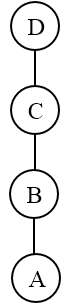
\includegraphics[scale = 1]{images/palm-aggregation-tree.png}\\
				\caption{Palm Shaped Aggregation Tree}
				\label{fig:Palm aggregation tree}
			\end{figure}
		The sensor node $C$ sends all the data-items in its payload with their signatures to its parent sensor node $D$.
		Furthermore, $C$ sends the signature of its payload $\textsf{Sign}_{S_{C}}(C_{0}||B_{1})$ to $D$.\\
			\begin{figure}[h!]
				\centering
				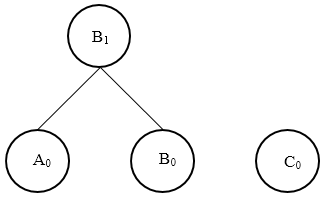
\includegraphics[scale = 1]{images/commitment-payload-of-C.png}
				\caption{$C$'s Commitment Payload}
				\label{fig:Commitment payload of C}
			\end{figure}
		\begin{equation}	
			\begin{array}{l}
				B_{1} =\ <B_{id}, 2, B_{1value}, H(N||2||B_{1value}||A_{0}||B_{0})>;\ \textsf{Sign}_{S_{B}}(B_{1})\\
				C_{0} =\ <C_{id}, 1, C_{value}, H(N||1||C_{value})>;\ \textsf{Sign}_{S_{C}}(C_{0})\\
				\textcolor{red}{\textsf{Sign}_{S_{C}}(C_{0}||B_{1})}
			\end{array}
			\label{eq:forwarding-payload-without-resigning}
		\end{equation}
	Signature on the $C$'s payload $\textsf{Sign}_{S_{C}}(C_{0}||B_{1})$ assures that the sensor node $C$ sent only two data-items $C_{0},B_{1}$ in its payload.
\section{Forwarding the Commitment Payload}	
	% This example showcases another important aspect of the protocol.
	% It shows two different ways of creating a commitment tree.
	The sensor node $C$ has two data-items $C_{0},B_{1}$ in its payload as shown in Equation \ref{eq:forwarding-payload-without-resigning}. 
	It sends the $\textsf{Sign}_{S_{B}}(B_{1})$, $\textsf{Sign}_{S_{C}}(C_{0}) $ and $\textsf{Sign}_{S_{C}}(C_{0}||B_{1})$ to its parent node $D$.
	It requires the parent node $D$ to know the public key of the sensor nodes $C$ and $D$, hence their certificates.
	Instead of that the sensor node $C$ can verify the $\textsf{Sign}_{S_{B}}(B_{1})$ then remove the old signature and create new signature $\textsf{Sign}_{S_{C}}(B_{1})$ signed by itself on the data-item $B_{1}$ as shown below:
\begin{equation}	
	\begin{array}{l}
		B_{1} =\ <B_{id}, 2, B_{1value}, H(N||2||B_{1value}||A_{0}||B_{0})>;\  \textcolor{red}{\textsf{Sign}_{S_{C}}(B_{1})}\\
		C_{0} =\ <C_{id}, 1, C_{value}, H(N||1||C_{value})>;\ \textsf{Sign}_{S_{C}}(C_{0})\\
		\textsf{Sign}_{S_{C}}(C_{0}||B_{1})
	\end{array}
	\label{eq:forwarding-payload-with-resigning}
\end{equation}
We call these two approaches \textbf{Forwarding signatures without resigning the data-items}, \textbf{Forwarding signatures with resigning the data-items} as shown in Equations \ref{eq:forwarding-payload-without-resigning} and \ref{eq:forwarding-payload-with-resigning} respectively .

To give an analogy with the real world application consider the following example.
One want to buy a diamond from the local diamond retailer.
Diamond is an expensive commodity so the end customer wants to verify its authenticity and integrity before purchasing.
Suppose, the diamond was created by the manufacturer in Africa, it was sold to a national wholesaler in the United States. 
The national wholesaler sells it to the state level reseller and he sells it to the city or county level retailer from whom the customer purchases the commodity.

One approach to verify the authenticity of the commodity is to make each entity in the supply chain to verify all the signatures on the received entity and sign on top of it.
And then forward the commodity with all the signatures to the next entity in the supply chain.
The next entity repeats the same procedure.
Hence, any entity in the supply chain need to verify the signatures of all its descendants in the supply chain.
In our example, it means to make the manufacturer from Africa signs the diamond and sells the signed diamond with his certificate.
The national level wholesaler in United States verifies the signature from the manufacturer using manufacturer's certificate.
Then he adds his signature and certificate, and sells to the state level reseller the diamond signed with two signatures and two certificates.
The state level reseller verifies both the signatures on the diamond using the certificates.
Then he adds his signature and certificate, and sells to the city level retailer the diamond singed with three signatures and three certificates. 
The city level retailer does the same thing before selling the diamond to the end customer.
In the end, the customer needs to verify all four signatures, using the received certificates.

% Note: that the same diamond now has been signed by four different entities. And the end customer need to know the certificate of all four parties to verify all those signatures.

An alternative approach to verify the authenticity of the commodity is to make each entity in the supply chain verify the signature, throw away the old signature, and then add its own signature on it. 
It means the next entity in the supply chain need to verify only a single signature.
The next entity repeats the same procedure.
Hence, any entity in the supply chain need to verify the signature of only its direct peer in the supply chain. 
In our example, it means to make the manufacturer from Africa signs the diamond and sells the signed diamond with his certificate.
The national level wholesaler in United States verifies the signature from the manufacturer using the manufacturer's certificate.
Then he removes the signature of the manufacturer, adds his own signature and certificate, and sells to the state level reseller the diamond signed with one signature and one certificate.
The state level reseller verifies only the signature from the wholesaler using the wholesaler's certificate.
Then he removes the signature of the wholesaler, adds his own signature and certificate, and sells to the city level retailer the diamond signed with one signature and one certificate.
The city level retailer does the same thing before selling the diamond to the end customer.
In the end, the customer needs to verify only one signature of the city level retailer using retailer's certificate.
This approach requires very few number of certificates overall in the supply chain.

Both theapproaches have their pros and cons and the perfect approach depends heavily on the application.
The various aspects of both the approaches for sensor nodes are discussed in the following sections.

	\section{\textcolor{red}{Forwarding signatures with resigning the data-items}}
		If we throw away the old signatures and resign the data-item with current aggregate node then following is true:
			\begin{itemize}
				\item Each parent needs the certificates of only its direct children.
				\item Each child needs to know the certificate of its parent only.
				\item Number of signatures remain the same as previous approach.
				\item Number of certificates needed in the network is $O(n)$; n is the number of nodes in the network.
				\item We do not need the signature of the payload.
			\end{itemize}

		% Analysis model:	
		% 	While creating CT;While distributing off-path; Both places together\\
		% Initial analysis says, if a single aggregate node cheats while CT generation or distributing off-path values it gets caught. 
		Note that we send signatures while distributing off-path values.
	\section{\textcolor{red}{Forwarding signatures without resigning the data-items}}

	\section{Commitment Tree Generation}
	For the given aggregation tree the commitment forest is built as follows.
	Leaf sensor nodes in the aggregation tree create their leaf vertex by creating data-items and their respective signatures according to Equation \ref{eq:leaf-vertex}, \ref{eq:signature-leaf-vertex} which they send it to their parent as a payload in the aggregation tree.
	Each internal sensor node $I$\ in the aggregation tree also creates their leaf vertex and its signature.
	In addition, $I$\ receives the payload from each of its children which creates the forest for $I$.
	Once $I$ verifies all the received signatures, it merges all the data-items in its forest with same count value to create its payload.
	Note that we can determine the height of the commitment tree from the count value.

	Suppose $I$ have to create its payload by merging $i$ data-items $D_{1}$, $D_{2}$, $\dotsc$, $D_{i}$ in its forest.
	First, $I$ verifies the received signatures $Sign(D_{1})$, $Sign(D_{2})$, $\dotsc$, $Sign(D_{i})$.
	Once verified, $I$ starts merging the data-items as follows.
	Let $c$ be the smallest count value in $I$'s forest.
	The sensor node $I$ finds two data-items $D_{1},D_{2}$ in its forest with the same count value $c$ and merges them into a new data-item with the count of $c+1$ as shown in Figure \ref{fig:increase-height}.
	\begin{figure}[h!]
		% \centering
		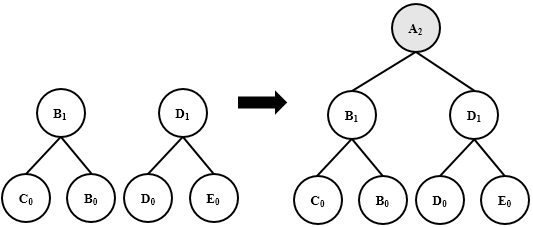
\includegraphics[width=6in]{images/increase-height.png}\\
		\caption{$A$ has $B_{1}, C_{1}$ in his forest and aggregates those two trees and creates $A_{2}$.}
		\label{fig:increase-height}
	\end{figure}\\
	It repeats the process until no two data-items in its forest have the same count value.
	An example of generating the payload by merging the data-items in the forest for the sensor node $A$ in Figure \ref{fig:at} is illustrated in the following example.
	% \ref{fig:commitment-tree-example-1}, \ref{fig:commitment-tree-example-2}, \ref{fig:commitment-tree-example-3}, \ref{fig:commitment-tree-example-4}.
			\begin{exmp} The commitment-payload generation process for node $A$ of Figure \ref{fig:at} is shown here.\\
				\begin{figure}[h!]
					\centering
					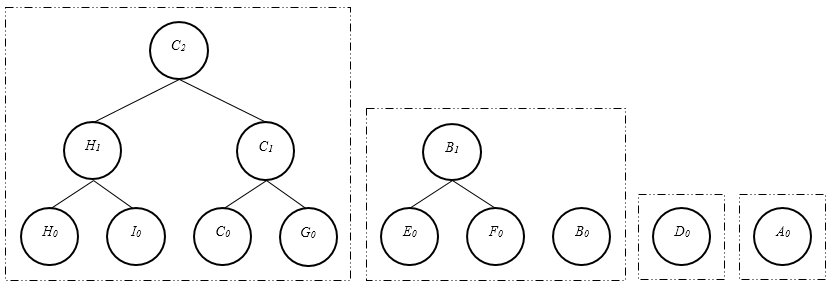
\includegraphics[width=6in]{images/commitment-tree-example-1.png}\\
					\caption{$A$ receives $C_{2}$ from $C$, $(B_{1},B_{0})$ from $B$, $D_{0}$ from $D$ and generates $A_{0}$. The commitment payload received from a given sensor node is indicated by dashed-line box.}
					\label{fig:commitment-tree-example-1}
				\end{figure}
				\begin{equation}
					\begin{array}{l}
						A_{0} = <A_{id}, 1, A_{value}, H(N||1||A_{value})>; \textsf{Sign}_{S_{A}}(A_{0}) \\
						D_{0} = <D_{id}, 1, D_{value}, H(N||1||D_{value})>; \textsf{Sign}_{S_{D}}(D_{0})\\
						B_{0} = <B_{id}, 1, B_{value}, H(N||1||B_{value})>; \textsf{Sign}_{S_{B}}(B_{0})\\
						B_{1} = <B_{id}, 2, B_{value}, H(N||2||B_{value}||E_{0}||F_{0})>; \textsf{Sign}_{S_{B}}(B_{1})\\
						\textcolor{red}{\textsf{Sign}_{S_{B}}(B_{0} || B_{1}), benefits}\\
						C_{2} = <C_{id}, 4, C_{value}, H(N||4||C_{value})||H_{1}||C_{1})>; \textsf{Sign}_{S_{C}}(C_{2})\\
						\end{array}
				\end{equation}

				\begin{figure}[h!]
					\centering
					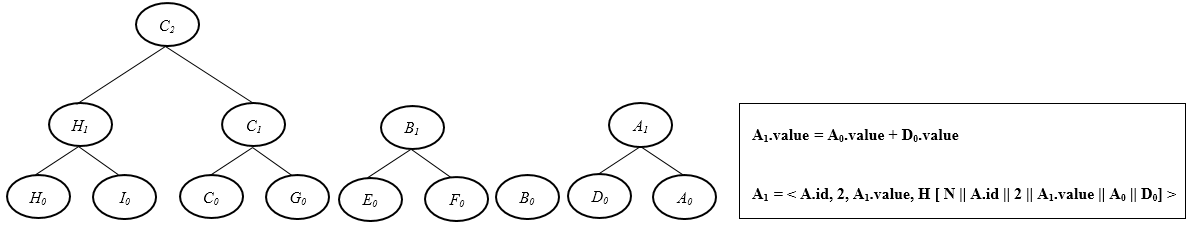
\includegraphics[width=6in]{images/commitment-tree-example-2.png}\\
					\caption{First Merge: $A_{1}$ vertex created by A.}
					\label{fig:commitment-tree-example-2}
				\end{figure}

				\begin{equation}
					\begin{array}{l}
				A_{1} = <A_{id}, 2, A_{1value}, H(N||2||A_{1value}||A_{0}||D_{0})>; \textsf{Sign}_{S_{A}}(A_{1})\\
				where\  A_{1value} = A_{value} + D_{value} \\
					\end{array}	
				\end{equation}
				\begin{figure}[h!]
					\centering
					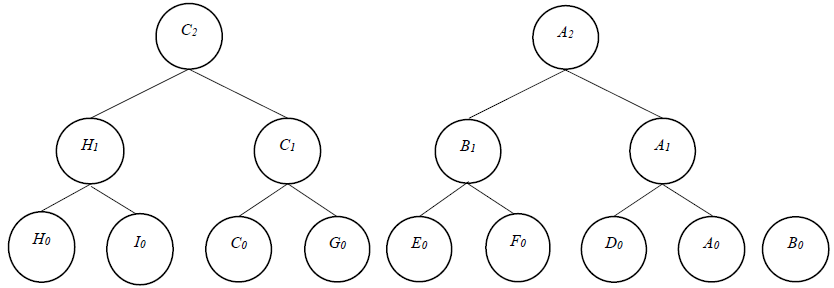
\includegraphics[width=\textwidth]{images/commitment-tree-example-3.png}\\
					\caption{Second Merge: $A_{2}$ vertex created by A.}
					\label{fig:commitment-tree-example-3}
				\end{figure}
				\begin{equation}
					\begin{array}{l}
						A_{2} = <A_{id}, 4, A_{2value}, H(N||4||A_{2value}||B_{1}||A_{1}) >; \textsf{Sign}_{S_{A}}(A_{2})\\
						where\  A_{2value} = B_{1value} + A_{1value} \\
					\end{array}
				\end{equation}
				\begin{figure}[h!]
					\centering
					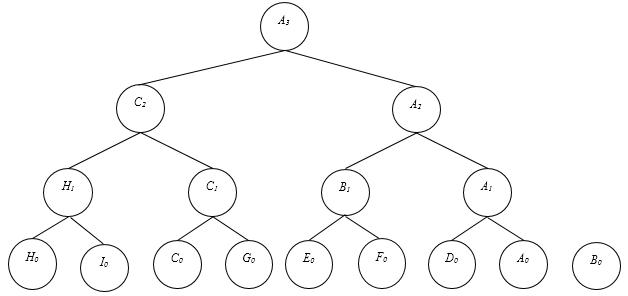
\includegraphics[width=6in]{images/commitment-tree-example-4.png}\\
					\caption{Third Merge: $A_{3}$ vertex created by A.}
					\label{fig:commitment-tree-example-4}
				\end{figure}
				\begin{equation}
					\begin{array}{l}
						A_{3} = <A_{id},8, A_{3value},H(N||8||A_{3value}||C_{2}||A_{2})>; \textsf{Sign}_{S_{A}}(A_{3})\\
						where\ A_{3value} = A_{2value} + C_{2value}
					\end{array}
				\end{equation}
			\end{exmp}
% chapter A Protocol for Commitment Tree Generation (end)

% Talk about the certificates:
	
% 	How many certificates does $A$ need to know in this example ?
% 	In the above example, $A$ need to know $D,B,C's$ certificate to verify their signatures.
% 	But if we use SHIA'a approach of creating commitment tree then $A$ need to know $E's$ certificate as well.
% 	Hence, being root in as many tree as possible is the more efficient.
\section{Bandwidth Analysis}
	For any given sensor node's forest with $n$ leaf vertices, has at most $\log n$ data-items in its payload.
	It has at most $(\log n) +1$ signatures in its payload.
	The highest possible count value is $\log n$, as all the trees are binary. 

	An intermediate sensor node $S$ with $\beta$ descendants in the aggregation tree, has at most $\log(\beta+1)$ data-items with their respective $\log(\beta+1)$ signatures in its payload.
	$S$ might need to send its payload signature $Sign(S_{p})$.
	At max, $S$ has to send a payload with $\log(\beta+1)$ data-items and $\log(\beta+1) +1$ signatures to its parent in the aggregation tree.
	
	Hence, sending signatures of the data-items causes $O(\log \beta)$ bandwidth overhead for each node in the network, where $\beta$ is the number of descendants of the sensor node. 
\section{Result checking}

\section{Performance Analysis}
	In addition to calculating its own data-items, all intermediate sensor nodes with $\beta$ descendants and $\zeta$ direct children need to do the following:
	\begin{itemize}
		\item To calculate and verify $O(\log \beta)$ signatures, creating $O(\log \beta)$ calculation overhead. 
		\item Needs sufficient memory to cache $O(\log \beta)$ certificates. 
		\item Needs enough memory to cache $\Omega(\zeta)$ certificates.
	\end{itemize}

	% Computation cost: Needs to calculate that many signatures. Needs to verify that many signatures.
	% Need to know that many certificates.

\section{Applications}
		The signature based aggregation scheme can be applied to do the \textbf{voting} in the network.
		And voting scheme can be used to solve many sensor network problems.
		For example, voting can be used to design the distributed algorithm for selecting a cluster head or node revocation system.
		In the voting scheme, following are the major security concerns: 
		\begin{itemize}
			\item The aggregate node needs to know that the vote is coming from the legit voter, no other voter is impersonating the vote of the legit voter.
			\item Only the intended aggregate node should be able to verify the vote.
			\item The aggregate node should not be able to tamper with the votes. 
			\item The aggregate node needs the proof that it aggregated the verified votes.
			\item The voter need the proof for which vote it sent to its aggregator.
		\end{itemize}
		For example, the base station wants to know the overall vote-count in the network.
		To do so, all the leaf nodes send their votes and the signature of their votes to their respective aggregate nodes in the network.
		The aggregate nodes receive votes with their signatures from all of their children voters.
		The aggregate nodes verify all the votes and count those votes.
		Then they forward the count and the signature of that count signed by the aggregate node to their respective parent in the aggregation tree.
		This process is repeated until the final count and its signature, is sent to the base station by the root of the aggregation tree.
				
	\textbf{Node power level},
	\textbf{Surveillance Application}
